%!TEX root = ../thesis.tex

\section{実験概要}
%\begin{figure}[hbtp]
  %\centering
 %\includegraphics[keepaspectratio, scale=0.8]
      %{images/RaspberryPiMouse.png}
 %\caption{Example}
 %\label{Fig:Example}
%\end{figure}
%\subsection{実験概要}
本研究では,本研究室で開発されているロボット ORNE-box3\cite{井口颯人2023屋外自律移動ロボットプラットフォーム-orne} を用いて走行実験を行った.実機ロボットの外観は\figref{Fig:ORNE-box3}に示す.ORNE-box3のセンサ構成については、\figref{Fig:sensor configuration}に示すように,PCとしてJetson Orin NX 16GBを搭載しており、3D LiDAR:R-Fans-16
、IMU:ADIS16465、Encoder : i-Cart middleを備えている.3D LiDARは、自己位置推定と障害物検知に使用し、IMUとエンコーダは、emcl2に対して情報を提供している.

走行ルートは\figref{Fig:Course map of the Tsudanuma Challenge 2025}が示すように,津田沼校舎2号館前から食堂前に設置されたコーンまでとし,
津田沼チャレンジのコースの一部を利用した.このルートは,屋外環境における
自律移動性能を評価するための実環境を想定したものである.


実験では,Navigation2 における各種パラメータを個別に変化させた場合の
ロボットの挙動の変化を調査することを目的とした.
各走行実験においては,対象とするパラメータのみを変更し,
それ以外のパラメータはすべて一定に保った.

また,パラメータの変更に際しては,変更前の設定値を基準値とし,
基準値から増減させた場合のロボットの走行挙動を比較・分析した.
これにより,各パラメータがロボットの走行安定性や挙動に与える影響を
明確にすることを試みた.

\begin{figure}[hbtp]
  \centering
 \includegraphics[keepaspectratio, scale=0.6]
      {images/tsudanumachallenge.png}
 \caption{Course map of the Tsudanuma Challenge 2025(source: \cite{Tsudanumachallenge})}
 \label{Fig:Course map of the Tsudanuma Challenge 2025}
\end{figure}

\begin{figure}[hbtp]
  \centering
 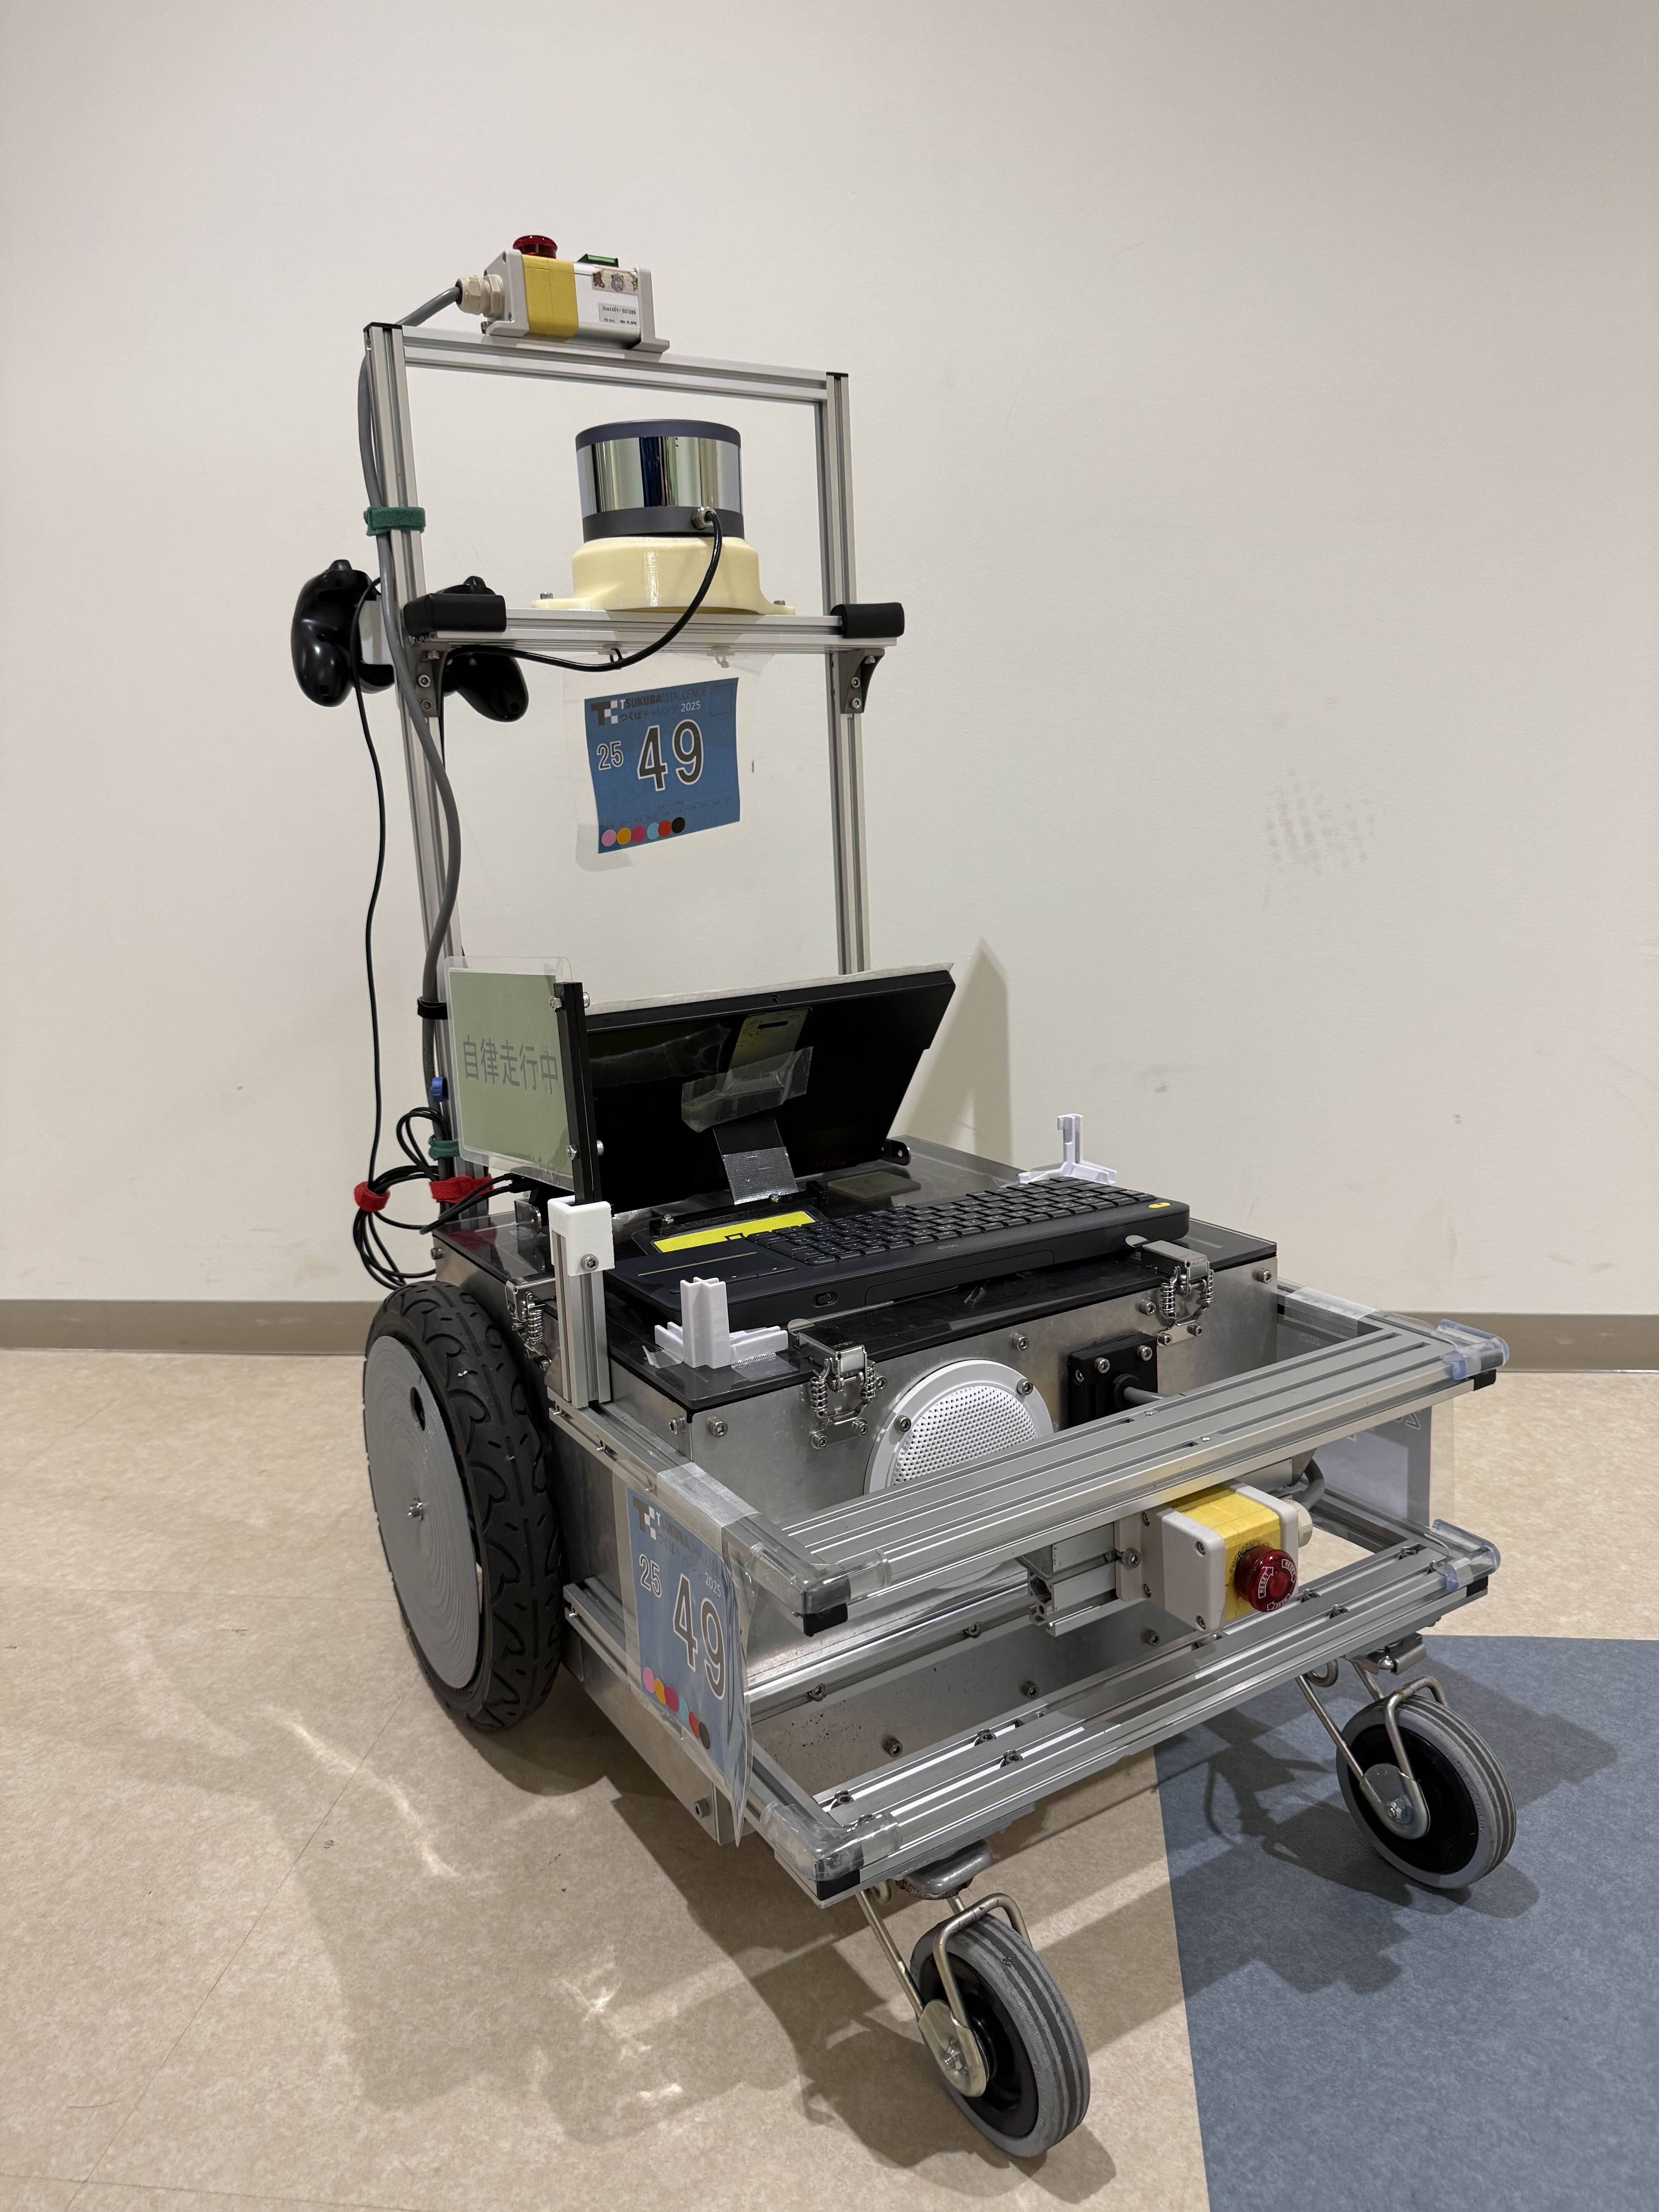
\includegraphics[keepaspectratio, scale=0.3]
      {images/orne-box3.png}
 \caption{ORNE-box3(source: \cite{井口颯人2023屋外自律移動ロボットプラットフォーム-orne})}
 \label{Fig:ORNE-box3}
\end{figure}
\begin{figure}[hbtp]
  \centering
 \includegraphics[keepaspectratio, scale=0.3]
      {images/sensor.png}
 \caption{sensor configuration}
 \label{Fig:sensor configuration}
\end{figure}
%\subsubsection{etc...}






\newpage

\section{実験結果}
%\begin{figure}[hbtp]
  %\centering
 %\includegraphics[keepaspectratio, scale=0.8]
      %{images/RaspberryPiMouse.png}
 %\caption{Example}
 %\label{Fig:Example}
%\end{figure}
\subsection{実験結果(emcl2)}
\subsubsection{実験結果(num\_particles)}

\begin{table}[H]
  \centering
  \caption{パーティクル数の違いによるゴール到達可否}
  \label{tab:num_particles_result}
  \begin{tabular}{c|c|c|c}
    \hline
    & \multicolumn{3}{c}{Number of particles} \\
    \hline
    number of times  & 200 & 500 (base) & 1000 \\
    \hline
    1  & $\times$ & ○ & ○ \\
    2  & ○ & ○ & $\times$ \\
    3  & $\times$ & $\times$ & $\times$ \\
    4  & ○ & ○ & ○ \\
    5  & ○ & ○ & $\times$ \\
    6  & $\times$ & $\times$ & $\times$ \\
    7  & ○ & ○ & ○ \\
    8  & ○ & ○ & ○ \\
    9  & ○ & ○ & ○ \\
    10 & ○ & ○ & ○ \\
    \hline
  \end{tabular}
\end{table}

Table\ref{tab:num_particles_result}に、パーティクル数の違いによるゴール到達の可否を示す.

\begin{table}[H]
  \centering
  \caption{パーティクル数ごとのゴール到達成功率}
  \label{tab:num_particles_success_rate}
  \begin{tabular}{c|c}
    \hline
    パーティクル数 & 成功率 [\%] \\
    \hline
    200  & 60 \\
    500 (base) & 80 \\
    1000 & 60 \\
    \hline
  \end{tabular}
\end{table}

Table\ref{tab:num_particles_success_rate}に,
パーティクル数を変化させた際のゴール到達成功率を示す.

Table\ref{tab:num_particles_result},Table\ref{tab:num_particles_success_rate}が示すように、パーティクル数を 200,500,1000 と変化させて自己位置推定の安定性を評価した.
その結果,パーティクル数 500 の場合に最も高いゴール到達率が得られた.
一方で,200 および 1000 の場合は,到達率がやや低下する傾向が確認された.
パーティクル数が少ないと自己位置推定が破綻しやすく、成功率が低下した.また、パーティクル数が多すぎても計算量の増加によって、遅延が発生して安定性が低下した。
以上より,パーティクル数は多ければ良いわけではなく,
自己位置推定の精度と計算負荷のバランスを考慮した適切な設定が重要であることが分かる.
本実験環境においては,パーティクル数 500 が最も安定した性能を示した.

次からの実験では、\figref{Fig:base orientation},\figref{Fig:base position}のグラフが基準の値の時のロボットの挙動である。\figref{Fig:base direction}はロボットの向き、\figref{Fig:base position}はロボットの位置のグラフである。
\begin{figure}[H]
  \centering
 \includegraphics[keepaspectratio, scale=0.65]
      {images/base_muki2.png}
 \caption{base orientation}
 \label{Fig:base orientation}
\end{figure}
\begin{figure}[H]
  \centering
 \includegraphics[keepaspectratio, scale=0.5]
      {images/base_postion.png}
 \caption{base position}
 \label{Fig:base position}
\end{figure}

\subsubsection{実験結果(odom\_fw\_dev\_per\_fw)}
\figref{Fig:base orientation},\figref{Fig:base position}で示すように基準の値は、0.19
\begin{figure}[H]
  \centering
 \includegraphics[keepaspectratio, scale=0.6]
      {images/fwfw0.01muki.png}
 \caption{Robot orientation with fw\_dev\_per\_fw = 0.01}
 \label{Fig:Robot orientation with fw_dev_per_fw = 0.01 }
\end{figure}
\begin{figure}[H]
  \centering
 \includegraphics[keepaspectratio, scale=0.6]
      {images/fwfw0.01iti.png}
 \caption{Robot position with fw\_dev\_per\_fw = 0.01
}
 \label{Fig:Robot position with fw_dev_per_fw = 0.01}
\end{figure}

\begin{figure}[H]
  \centering
 \includegraphics[keepaspectratio, scale=0.6]
      {images/fwfw0.05muki2.png}
 \caption{Robot orientation with fw\_dev\_per\_fw = 0.05}
 \label{Fig:Robot orientation with fw_dev_per_fw = 0.05 }
\end{figure}
\begin{figure}[H]
  \centering
 \includegraphics[keepaspectratio, scale=0.6]
      {images/fwfw0.05iti2.png}
 \caption{Robot position with fw\_dev\_per\_fw = 0.05
}
 \label{Fig:Robot position with fw_dev_per_fw = 0.05}
\end{figure}

\begin{figure}[H]
  \centering
 \includegraphics[keepaspectratio, scale=0.6]
      {images/fwfw0.1muki2.png}
 \caption{Robot orientation with fw\_dev\_per\_fw = 0.1}
 \label{Fig:Robot orientation with fw_dev_per_fw = 0.1 }
\end{figure}
\begin{figure}[H]
  \centering
 \includegraphics[keepaspectratio, scale=0.6]
      {images/fwfw0.1iti2.png}
 \caption{Robot position with fw\_dev\_per\_fw = 0.1
}
 \label{Fig:Robot position with fw_dev_per_fw = 0.1}
\end{figure}

\begin{figure}[H]
  \centering
 \includegraphics[keepaspectratio, scale=0.6]
      {images/fwfw0.3muki.png}
 \caption{Robot orientation with fw\_dev\_per\_fw = 0.3}
 \label{Fig:Robot orientation with fw_dev_per_fw = 0.3 }
\end{figure}
\begin{figure}[H]
  \centering
 \includegraphics[keepaspectratio, scale=0.6]
      {images/fwfw0.3iti.png}
 \caption{Robot position with fw\_dev\_per\_fw = 0.3
}
 \label{Fig:Robot position with fw_dev_per_fw = 0.3}
\end{figure}

\begin{figure}[H]
  \centering
 \includegraphics[keepaspectratio, scale=0.6]
      {images/fwfw0.4muki.png}
 \caption{Robot orientation with fw\_dev\_per\_fw = 0.4}
 \label{Fig:Robot orientation with fw_dev_per_fw = 0.4 }
\end{figure}
\begin{figure}[H]
  \centering
 \includegraphics[keepaspectratio, scale=0.6]
      {images/fwfw0.4iti.png}
 \caption{Robot position with fw\_dev\_per\_fw = 0.4
}
 \label{Fig:Robot position with fw_dev_per_fw = 0.4}
\end{figure}

\begin{figure}[H]
  \centering
 \includegraphics[keepaspectratio, scale=0.6]
      {images/fwfw0.5muki.png}
 \caption{Robot orientation with fw\_dev\_per\_fw = 0.5}
 \label{Fig:Robot orientation with fw_dev_per_fw = 0.5 }
\end{figure}
\begin{figure}[H]
  \centering
 \includegraphics[keepaspectratio, scale=0.6]
      {images/fwfw0.5iti.png}
 \caption{Robot position with fw\_dev\_per\_fw = 0.5
}
 \label{Fig:Robot position with fw_dev_per_fw = 0.5}
\end{figure}

\figref{Fig:Robot orientation with fw_dev_per_fw = 0.5 }で示すように、odom\_fw\_dev\_per\_fw を 0.5 に設定した場合,ロボットは走行を続けるにつれて自己位置推定の誤差が累積し,最終的にゴールに到達することができなかった.一方で,0.4 以下の値に設定した場合には,ロボットはゴールまで到達することが確認された.

また,直線走行時の挙動を基準条件と比較すると,odom\_fw\_dev\_per\_fw を大きく設定した場合には,推定されたロボットの位置が徐々にずれていく様子が確認された.このことから,odom\_fw\_dev\_per\_fw の値を過度に大きくすると,前進移動に対するオドメトリ誤差が強調され,自己位置推定の精度が低下することが示唆される.

%\figref{Fig:Robot orientation with fw_dev_per_fw = 0.01 },\figref{Fig:Robot position with fw_dev_per_fw = 0.01}

\subsubsection{実験結果(odom\_fw\_dev\_per\_rot)}
\figref{Fig:base orientation},\figref{Fig:base position}で示すように、基準の値は、0.0001

\begin{figure}[H]
  \centering
 \includegraphics[keepaspectratio, scale=0.6]
      {images/fwrot0.001muki.png}
 \caption{Robot orientation with fw\_dev\_per\_rot = 0.001}
 \label{Fig:Robot orientation with fw_dev_per_rot = 0.001 }
\end{figure}
\begin{figure}[H]
  \centering
 \includegraphics[keepaspectratio, scale=0.6]
      {images/fwrot0.001iti.png}
 \caption{Robot position with fw\_dev\_per\_rot = 0.001
}
 \label{Fig:Robot position with fw_dev_per_rot = 0.001}
\end{figure}

\begin{figure}[H]
  \centering
 \includegraphics[keepaspectratio, scale=0.6]
      {images/fwrot0.01muki.png}
 \caption{Robot orientation with fw\_dev\_per\_rot = 0.01}
 \label{Fig:Robot orientation with fw_dev_per_rot = 0.01 }
\end{figure}
\begin{figure}[H]
  \centering
 \includegraphics[keepaspectratio, scale=0.6]
      {images/fwrot0.01iti.png}
 \caption{Robot position with fw\_dev\_per\_rot = 0.01
}
 \label{Fig:Robot position with fw_dev_per_rot = 0.01}
\end{figure}

\begin{figure}[H]
  \centering
 \includegraphics[keepaspectratio, scale=0.6]
      {images/fwrot0.1muki.png}
 \caption{Robot orientation with fw\_dev\_per\_rot = 0.1}
 \label{Fig:Robot orientation with fw_dev_per_rot = 0.1 }
\end{figure}
\begin{figure}[H]
  \centering
 \includegraphics[keepaspectratio, scale=0.6]
      {images/fwrot0.1iti.png}
 \caption{Robot position with fw\_dev\_per\_rot = 0.1
}
 \label{Fig:Robot position with fw_dev_per_rot = 0.1}
\end{figure}

\begin{figure}[H]
  \centering
 \includegraphics[keepaspectratio, scale=0.6]
      {images/fwrot0.5muki.png}
 \caption{Robot orientation with fw\_dev\_per\_rot = 0.5}
 \label{Fig:Robot orientation with fw_dev_per_rot = 0.5 }
\end{figure}
\begin{figure}[H]
  \centering
 \includegraphics[keepaspectratio, scale=0.6]
      {images/fwrot0.5iti.png}
 \caption{Robot position with fw\_dev\_per\_rot = 0.5
}
 \label{Fig:Robot position with fw_dev_per_rot = 0.5}
\end{figure}

odom\_fw\_dev\_per\_rot を変化させた実験では,すべての設定値においてロボットはゴールに到達することができた.特に,odom\_fw\_dev\_per\_rot を 0.5 に設定した場合には,走行中に自己位置推定のずれが一部確認されたものの,走行不能となるような大きな影響は見られず,最終的にゴールまで到達することが確認された.

この結果から,odom\_fw\_dev\_per\_rot は自己位置推定に一定の影響を与えるものの,fw 方向の移動誤差を表す odom\_fw\_dev\_per\_fw と比較すると,ゴール到達性に与える影響は相対的に小さいと考えられる.


\subsubsection{実験結果(odom\_rot\_dev\_per\_fw)}
\figref{Fig:base orientation},\figref{Fig:base position}で示すように基準の値は、0.13

\begin{figure}[H]
  \centering
 \includegraphics[keepaspectratio, scale=0.6]
      {images/rotfw0.01muki.png}
 \caption{Robot orientation with rot\_dev\_per\_fw = 0.01}
 \label{Fig:Robot orientation with rot_dev_per_fw = 0.01 }
\end{figure}
\begin{figure}[H]
  \centering
 \includegraphics[keepaspectratio, scale=0.6]
      {images/rotfw0.01iti.png}
 \caption{Robot position with rot\_dev\_per\_fw = 0.01
}
 \label{Fig:Robot position with rot_dev_per_fw = 0.01}
\end{figure}

\begin{figure}[H]
  \centering
 \includegraphics[keepaspectratio, scale=0.6]
      {images/rotfw0.2muki.png}
 \caption{Robot orientation with rot\_dev\_per\_fw = 0.2}
 \label{Fig:Robot orientation with rot_dev_per_fw = 0.2 }
\end{figure}
\begin{figure}[H]
  \centering
 \includegraphics[keepaspectratio, scale=0.6]
      {images/rotfw0.2iti.png}
 \caption{Robot position with rot\_dev\_per\_fw = 0.2
}
 \label{Fig:Robot position with rot_dev_per_fw = 0.2}
\end{figure}

\begin{figure}[H]
  \centering
 \includegraphics[keepaspectratio, scale=0.6]
      {images/rotfw0.3muki.png}
 \caption{Robot orientation with rot\_dev\_per\_fw = 0.3}
 \label{Fig:Robot orientation with rot_dev_per_fw = 0.3 }
\end{figure}
\begin{figure}[H]
  \centering
 \includegraphics[keepaspectratio, scale=0.6]
      {images/rotfw0.3iti.png}
 \caption{Robot position with rot\_dev\_per\_fw = 0.3
}
 \label{Fig:Robot position with rot_dev_per_fw = 0.3}
\end{figure}

\begin{figure}[H]
  \centering
 \includegraphics[keepaspectratio, scale=0.6]
      {images/rotfw0.4muki.png}
 \caption{Robot orientation with rot\_dev\_per\_fw = 0.4}
 \label{Fig:Robot orientation with rot_dev_per_fw = 0.4 }
\end{figure}
\begin{figure}[H]
  \centering
 \includegraphics[keepaspectratio, scale=0.6]
      {images/rotfw0.4iti.png}
 \caption{Robot position with rot\_dev\_per\_fw = 0.4
}
 \label{Fig:Robot position with rot_dev_per_fw = 0.4}
\end{figure}

\begin{figure}[H]
  \centering
 \includegraphics[keepaspectratio, scale=0.6]
      {images/rotfw0.5muki.png}
 \caption{Robot orientation with rot\_dev\_per\_fw = 0.5}
 \label{Fig:Robot orientation with rot_dev_per_fw = 0.5 }
\end{figure}
\begin{figure}[H]
  \centering
 \includegraphics[keepaspectratio, scale=0.6]
      {images/rotfw0.5iti.png}
 \caption{Robot position with rot\_dev\_per\_fw = 0.5
}
 \label{Fig:Robot position with rot_dev_per_fw = 0.5}
\end{figure}

rot\_dev\_per\_fwでの実験では、rot\_dev\_per\_fw の値を大きくした場合においても,ロボットは直進走行中に自己位置および姿勢のわずかなずれが生じるのみであり,走行不能となることはなく,最終的にゴールまで問題なく到達することが確認された.

直線走行区間(目標方位 270°)でのロボットの向きに着目すると,rot\_dev\_per\_fw を 0.01 に設定した\figref{Fig:Robot orientation with rot_dev_per_fw = 0.01 }の場合には,ロボットは目標方位をほぼ維持したまま高い精度で直進していることが確認できた.一方で,rot\_dev\_per\_fw を 0.4 以上に設定した\figref{Fig:Robot orientation with rot_dev_per_fw = 0.4 },\figref{Fig:Robot orientation with rot_dev_per_fw = 0.5 }で示した場合には,走行中のロボットの方位が 270° を下回る傾向が見られ,進行に伴って姿勢が徐々にずれていく様子が確認された.

しかしながら,この方位のずれはナビゲーション全体に致命的な影響を与えるほどではなく,ゴール到達性に大きな影響は見られなかった.


\subsubsection{実験結果(odom\_rot\_dev\_per\_rot)}
\figref{Fig:base orientation},\figref{Fig:base position}で示すように基準の値は、0.19



\subsubsection{実験結果(laser\_likelihood\_max\_dist)}

\subsubsection{実験結果(range\_threshold)}

\subsection{実験結果(Nav2\_controller)}

\subsubsection{実験結果(max\_vel\_x)}

\subsubsection{実験結果(max\_vel\_theta)}

\subsubsection{実験結果(max\_speed\_xy)}

\subsubsection{実験結果(min\_theta\_velocity\_threshold)}

\subsubsection{実験結果(acc\_lim\_x)}

\subsubsection{実験結果(acc\_lim\_theta)}

\subsection{実験結果(Nav2\_Costmap)}

\subsubsection{実験結果(global\_resolution)}

\subsubsection{実験結果(global\_cost\_scaling\_factor)}

\subsubsection{実験結果(global\_inflation\_radius)}

\subsubsection{実験結果(local\_resolution)}

\subsubsection{実験結果(local\_cost\_scaling\_factor)}

\subsubsection{実験結果(local\_inflation\_radius)}

\subsection{実験結果(Nav2\_Velocity Smoother)}

\subsubsection{実験結果(smoothing\_frequency)}

\subsubsection{実験結果(max\_velocity)}

\subsubsection{実験結果(max\_accel\_ms)}

\subsubsection{実験結果(max\_accel\_rads)}

\subsection{実験結果(Nav2\_planner goal)}

\subsubsection{実験結果(linear\_granularity)}

\subsubsection{実験結果(angular\_granularity)}

\subsubsection{実験結果(xy\_goal\_tolerance)}

\subsubsection{実験結果(trans\_stopped\_velocity)}

\subsubsection{実験結果(planner\_tolerance)}


%\subsubsection{etc...}